\chapter{State of the art}

\section{MyRobotLab}

MyRobotLab is a framework that provides controllers and functionality to robotics projects, most
relevant of which being the OpenCV computer vision service and the user interface to use it.
It provides access to OpenCV specific image filters, that are applied as ``pipeline filters`` through
the MyRobotLab interface. ``Some filters have configuration which can be changed``, leading to a
streamlined learning experience and emphasis on interactivity. \cite{myRobotLab}

For the upside of providing and entire framework that encompasses all facets of robotics software
design, MyRobotLab greatest downside as a learning tool is the lack of explanations. While being
and excellent tool for the average robotics enthusiast to further their own knowledge, it does little
to help the novice user. Most of the explanation is given as external resources, as opposed to
in-application information.

\begin{figure}[H]
	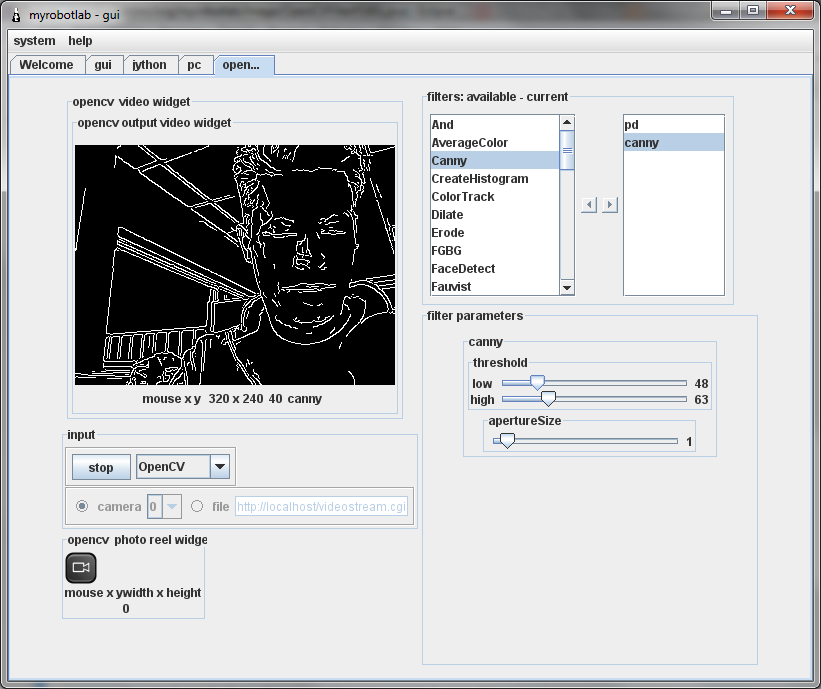
\includegraphics[width=0.9\textwidth, height=0.65\textwidth]{myrobotlab}
	\caption{Canny filter and parameters in MyRobotLab \cite{myRobotLab}}
\end{figure}


\section{OpenCV Demonstrator}

Provided by the creators of the OpenCV Library, the demonstrator is a ``allows one to select an image
processing function [...] and then a demonstration of the function automatically displays``.
It also provides the ability programmatically to change filter parameters, and is intended as a showcase
for all OpenCV features, serving as a way to ``explore different image processing functions included in 
OpenCV, without having to write a single line of code``. \cite{opencvDemo}

Although a myriad of possible image modifications is provided, each with a dedicated in-app explination,
they can only be showcased individually.
While this serves well for a library demonstration, it is only siuted for understanding the modules
provided by OpenCV, and not as a fully-fledged learning experience, as it lacks the delpth provided
by mixing and matching different filters in order to gauge the interactions between them.

\begin{figure}[H]
	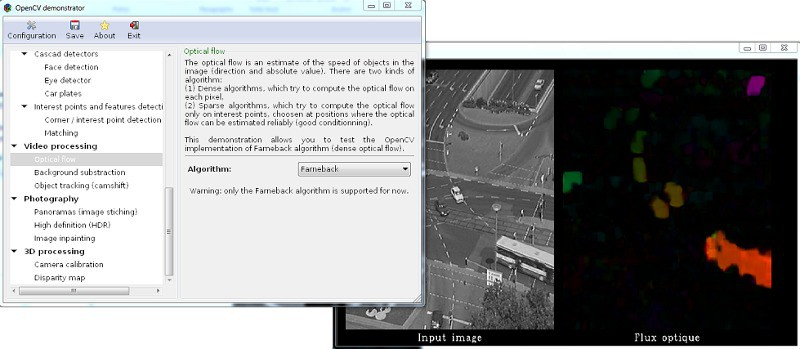
\includegraphics[width=0.9\textwidth, height=0.65\textwidth]{opencvDemo}
	\caption{OpenCV Demonstrator - User interface \cite{opencvDemo}}
\end{figure}

